\section{三类积分之间的关系}
\label{sec:multivariable-boundary-relations}

一元微积分基本定理把导数在区间上的积分化为两个端点的函数值之差。
区域、路径和曲面积分也有类似关系：特定导数在内部的积分，可以化为原函数或原向量场在边界上的积分。
本节分别回答三个问题：平面区域积分何时等于边界路径积分，空间区域积分何时等于边界曲面积分，曲面积分何时等于边界路径积分。

这些关系中的被积对象不能互换。路径环流累计向量场的切向分量，通量累计向量场的法向分量；
相应的内部积分分别使用旋度或散度。下面先明确这些导数的输入与输出，以及边界方向的约定，再给出各公式的条件与推导。
所有区域积分以及路径、曲面的参数积分均采用勒贝格积分。经典公式的组织参考向量微积分教材\scite{math-openstax-calculus3}。

\subsection{积分公式中的微分算子}

前面已用梯度表示多元标量函数的一阶变化。现在给定开集$U$上的向量场$\bm F$，我们关心它的各分量怎样共同产生净流出或环流。
这两个问题需要不同的偏导数组合。先介绍以向量场为输入的散度与旋度，再介绍以标量函数为输入的Laplace算子，分别明确它们的输出类型。

\subsubsection{散度}

对一个小长方体，沿每个坐标方向流出的量与流入的量之差，取决于向量场在该方向上的分量怎样变化。
把各坐标方向的变化率相加，就得到描述局部净流出的标量。
\begin{definition}[散度]
\label{def:multivariable-divergence}
设$U\subseteq\mathbb R^d$为开集，$\bm F=(F_1,\ldots,F_d)^\top:U\to\mathbb R^d$的各分量一阶偏导数存在。
$\bm F$的\term{散度}（divergence）是标量函数
\[
 \operatorname{div}\bm F
 =\nabla\mathbin{\cdot}\bm F
 =\sum_{j=1}^d\partial_jF_j.
\]
\end{definition}
三维径向场$\bm F(x,y,z)=(x,y,z)^\top$的散度是$1+1+1=3$；
旋转场$\bm G(x,y,z)=(-y,x,0)^\top$的散度是$0$。
散度为零表示局部净流出率为零，并不表示向量场为零。
二维场$(P,Q)^\top$的散度相应为$P_x+Q_y$，后面的平面通量公式使用这一标量函数。

\subsubsection{旋度}

净流出不能描述绕一点旋转的运动：上面的旋转场散度为零，沿圆周的环流却不为零。
在三维空间中，需要分别记录绕三个坐标方向的局部环流率，并把它们组成一个向量。
\begin{definition}[旋度]
\label{def:multivariable-curl}
设$U\subseteq\mathbb R^3$为开集，$\bm F=(F_1,F_2,F_3)^\top:U\to\mathbb R^3$的各分量一阶偏导数存在。
$\bm F$的\term{旋度}（curl）是向量场
\[
 \operatorname{curl}\bm F=\nabla\times\bm F
 =\begin{pmatrix}
   \partial_yF_3-\partial_zF_2\\
   \partial_zF_1-\partial_xF_3\\
   \partial_xF_2-\partial_yF_1
  \end{pmatrix}.
\]
\end{definition}
例如$\bm F=(-y/2,x/2,0)^\top$的旋度为$(0,0,1)^\top$，径向场$(x,y,z)^\top$的旋度为零。
旋度沿某一单位法向的分量，描述垂直于该方向的小曲面上的局部环流率；后面的Stokes公式把这一关系写成积分等式。

对二维场$(P,Q)^\top$，平面内需要的是标量$Q_x-P_y$。
将它补零写成三维场$(P,Q,0)^\top$后，这一标量正是旋度的第三分量，因而与向上法向相对应。
符号$\nabla\mathbin\cdot$和$\nabla\times$表示这里定义的偏导数组合，不是两个普通数值向量的内积或叉积。


图~\ref{fig:analysis-process-divergence-circulation-fields}在同一个单位圆周上分别观察净流出与切向环流，比较两种微分算子所记录的信息。
\begin{figure*}[!htbp]
 \centering
 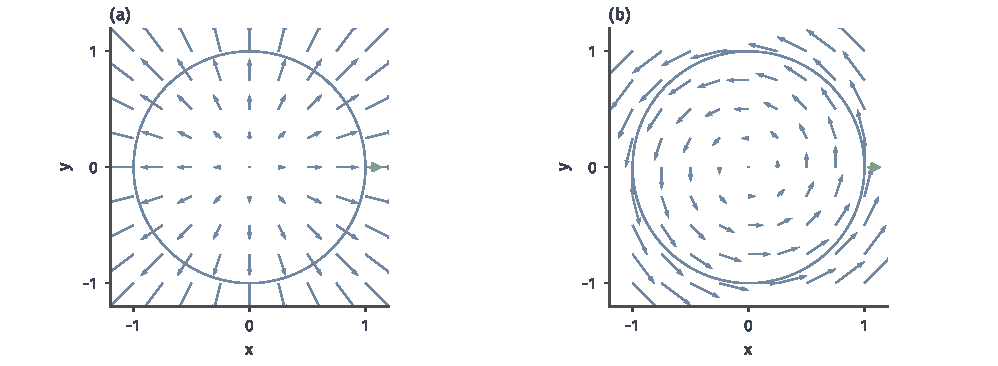
\includegraphics[width=169.0mm]{figures/01-mathematical-preliminaries-upper/01-mathematical-language-combinatorics-analysis-optimization/matplotlib/chapter3-concept-processes/divergence-circulation-fields.pdf}
 \caption{(a) 径向场$(x,y)^\top$的二维散度为$2$、旋转率$Q_x-P_y=0$，圆周外向通量为$2\pi$、环流为零。(b) 旋转场$(-y,x)^\top$的散度为零、旋转率为$2$，通量为零、环流为$2\pi$。绿箭头仅标记外法向；蓝色场箭头按相同常数缩放。零散度不等于零场，也不等于零环流。}
 \label{fig:analysis-process-divergence-circulation-fields}
\end{figure*}

\subsubsection{Laplace算子}

标量函数的梯度是向量场，因此可以继续取散度，把各坐标方向的二阶变化相加。
这一复合运算在多元分部积分中出现，仍以标量函数作为输入与输出。
\begin{definition}[Laplace算子]
\label{def:multivariable-laplacian}
对开集$U\subseteq\mathbb R^d$上的二阶连续可微标量函数$v$，定义\term{Laplace算子}（Laplacian）为
\[
 \Delta v=\operatorname{div}(\nabla v)
 =\sum_{j=1}^d\partial_j^2v.
\]
\end{definition}
例如$v(x,y,z)=x^2+y^2+z^2$时，$\Delta v=6$。
梯度将标量函数变为向量场，散度将向量场变为标量函数；不能将$\Delta v$与向量场的旋度混为同一类对象。

\subsection{边界的定向}

将一个区域分成相邻小块时，公共边或公共面不属于原区域的外边界。
要使这些内部贡献相消，各小块必须采用相容的方向。不同几何对象的方向约定如下。

\subsubsection{平面区域的正向边界}

平面区域的边界是路径，所以先规定沿边界行进的方向。简单闭曲线指除首尾相合外不自交的闭曲线。
对有界平面区域，取边界方向使沿曲线前进时区域总在左侧，称为正向边界。
外边界因此逆时针，围绕孔洞的内边界顺时针。例如圆环$1<x^2+y^2<4$的两圈边界必须取相反方向。

边界由多段光滑弧组成时，按这一方向逐段相接，转角处不另加积分项。
相邻平面小块各自采用正向边界时，共同边被沿相反方向走过，两个有向路径积分恰好抵消。

\subsubsection{区域边界的外法向}

通量需要的是法向，而不是边界的行进方向。空间区域的外单位法向从内部指向外部；
有孔洞时，孔洞边界的外法向指向孔洞。相邻子区域的公共面上，各自的外法向相反，所以内部通量相消。
二维区域边界上的外单位法向也按同样方式规定，但积分按弧长累计。

\subsubsection{定向曲面边界的诱导方向}

曲面取定单位法向$\bm n$后，其边界路径的方向不能再任意选择。
边界正向按右手约定确定：右手大拇指朝法向，其余手指弯曲的方向为正向。
等价地，沿边界前进并把头朝向法向时，曲面留在左侧。向上定向的平面圆盘，其边界从上方看为逆时针。

若翻转曲面法向，边界的诱导方向也随之翻转。分片曲面的定向相容，指相邻曲面片在公共边上诱导出相反的行进方向。
这时公共边上的路径积分相消，只留下整张曲面的真正边界。


图~\ref{fig:analysis-process-boundary-orientation-cancellation}把相容方向的作用画出来：内边相消，才会只剩整个对象的外边界。
\begin{figure}[!htbp]
 \centering
 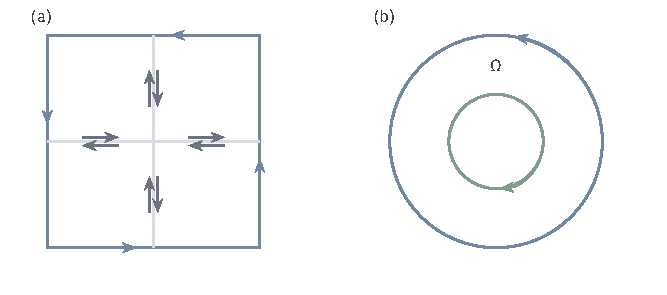
\includegraphics[width=112mm]{figures/01-mathematical-preliminaries-upper/01-mathematical-language-combinatorics-analysis-optimization/tikz/chapter3-concept-processes/boundary-orientation-cancellation.pdf}
 \caption{(a) 四个小正方形各取逆时针正向，共同边被沿相反方向走过；灰箭头略错开以便辨认，实际是同一条边。相加后只留下蓝色外边界。(b) 圆环的外边界逆时针、孔洞边界顺时针，沿任一边界前进时区域均在左侧。曲面拼片时也按公共边相反方向保证Stokes边界项相消。}
 \label{fig:analysis-process-boundary-orientation-cancellation}
\end{figure}

\subsection{平面区域积分与边界路径积分}

在平面上，区域的边界是一维路径。对同一个二维向量场，可以沿边界累计切向作用，也可以累计法向通量；
两种边界积分分别对应区域内部不同的偏导数组合。

\subsubsection{Green公式的环流形式}

沿正向边界的切向路径积分描述环流。它所对应的内部量是$Q_x-P_y$，而不是散度$P_x+Q_y$。
下面的公式把二者联系起来，并明确区域、场与方向的条件。
\begin{theorem}[Green公式]
\label{thm:multivariable-green}
设$\Omega\subseteq\mathbb R^2$为有界开区域，边界由有限条分段$C^1$简单闭曲线组成，
且区域在每段光滑边界附近位于边界的一侧。边界取正向，即外边界逆时针、孔洞边界顺时针。
若二维向量场$\bm F=(P,Q)^\top$在$\overline\Omega$的开邻域内连续可微，则\term{Green公式}（Green's theorem）给出
\begin{equation}
 \oint_{\partial\Omega}P\,\mathrm dx+Q\,\mathrm dy
 =\iint_\Omega\left(\frac{\partial Q}{\partial x}-\frac{\partial P}{\partial y}\right)\,\mathrm dx\,\mathrm dy.
 \label{eq:multivariable-green}
\end{equation}
\end{theorem}
左侧是向量场的切向路径积分；右侧是标量函数$Q_x-P_y$的区域积分。
在矩形上，二者的等式可以直接由一元基本定理和Fubini定理推出。
\begin{proof}[矩形情形的证明]
取$\Omega=(a,b)\times(c,d)$。场在闭矩形附近连续可微，以下被积函数均可积，故
\[
 \begin{aligned}
 -\iint_\Omega\partial_yP\,\mathrm dx\,\mathrm dy
 &=\int_a^b[P(x,c)-P(x,d)]\,\mathrm dx,\\
 \iint_\Omega\partial_xQ\,\mathrm dx\,\mathrm dy
 &=\int_c^d[Q(b,y)-Q(a,y)]\,\mathrm dy.
 \end{aligned}
\]
第一行对应下边从左向右、上边从右向左的两项积分，第二行对应右边从下向上、左边从上向下的两项积分。
四项合起来，正是沿下、右、上、左四条边逆时针行进得到的路径积分。
\end{proof}
有限个矩形拼接时，公共边上的积分因方向相反而抵消。
一般规则区域的证明还需处理区域分片及边界逼近误差，不能仅凭小矩形上的等式完成；这里引用一般形式，完整论证可参考向量微积分教材\scite{math-strang1991calculus}。

取$\bm F=(-y,x)^\top$、$\Omega$为单位圆盘，右侧被积函数为$2$，所以边界环流为$2\pi$。
这与直接参数化圆周得到的结果一致，也说明正向约定决定了结果的符号。

\subsubsection{Green公式的通量形式}

要计算穿过平面区域边界的净通量，需要把场投影到外法向上。
沿正向边界，单位切向量顺时针转过直角就得到外单位法向，因此它们的有向弧长分量满足
\[
 \bm n\,\mathrm ds=(\mathrm dy,-\mathrm dx)^\top.
\]
这一关系将法向通量转化为可以使用Green公式的路径积分。
\begin{theorem}[平面区域的通量公式]
\label{thm:multivariable-planar-flux}
在Green公式相同的区域条件下，若$\bm F=(F_1,F_2)^\top$在$\overline\Omega$的开邻域内连续可微，
$\bm n$是边界的外单位法向，则
\[
 \int_{\partial\Omega}\bm F^\top\bm n\,\mathrm ds
 =\iint_\Omega\operatorname{div}\bm F\,\mathrm dx\,\mathrm dy.
\]
\end{theorem}
\begin{proof}
利用外法向与正向边界的关系，左侧等于
$\oint_{\partial\Omega}(-F_2)\,\mathrm dx+F_1\,\mathrm dy$。
在Green公式中取$(P,Q)=(-F_2,F_1)$，右侧即为$\partial_xF_1+\partial_yF_2=\operatorname{div}\bm F$的区域积分。
\end{proof}
这也是二维的散度公式。它与环流形式使用相同的区域条件，但累计的边界分量和内部导数不同。

例如单位圆盘上的$\bm F(x,y)=(x,y)^\top$有散度$2$，区域积分为$2\pi$。
边界参数化为$\bm\gamma(t)=(\cos t,\sin t)^\top$，$0\leq t\leq2\pi$，
外法向$\bm n=\bm\gamma(t)$，$\mathrm ds=\mathrm dt$，且$\bm F^\top\bm n=1$，所以边界通量也为$2\pi$。
若改取内法向，通量就变为$-2\pi$。
相比之下，旋转场$(-y,x)^\top$的散度为零，在圆周上与法向垂直，通量为零；它的环流却是前面算出的$2\pi$。

\subsection{空间区域积分与边界曲面积分}

将平面区域换成三维空间区域后，边界从曲线变成闭曲面。
对应关系仍然是内部散度的积分等于边界净通量；这一关系还可以推出多元函数的分部积分公式。

\subsubsection{Gauss公式}

一个小长方体的两张相对面分别记录某一分量的流出与流入。一元基本定理把两者之差写成该分量偏导数的体积积分。
三个坐标方向相加，就得到散度与闭曲面通量之间的关系。
\begin{theorem}[Gauss散度定理]
\label{thm:analysis-divergence-theorem}
设$\Omega\subseteq\mathbb R^3$为有界开区域，其边界是由有限个正则$C^1$曲面片组成的闭曲面。
各片内部互不相交，接缝为有限条分段$C^1$曲线及有限个点；在每个光滑边界点附近，区域位于边界的一侧。
若向量场$\bm F$在$\overline\Omega$的一个开邻域内连续可微，则\term{散度定理}（divergence theorem）给出
\begin{equation}
  \int_{\Omega}\nabla\mathbin{\cdot}\bm F\,\mathrm d\bm x
  =\int_{\partial\Omega}\bm F^\top\bm n\,\mathrm dS,
 \label{eq:analysis-divergence-theorem}
\end{equation}
其中$\bm n$是光滑边界片上的外单位法向，$\mathrm dS$为面积元素。
\end{theorem}
光滑有界区域和通常的多面体满足这些条件。接缝的曲面面积为零，不影响通量积分；所列条件也保证两侧积分有限。
左侧累计向量场的局部净流出率，右侧累计穿过整个外边界的净通量。

对长方体，这一等式不需要借助一般曲面逼近，可以逐坐标证明。
\begin{proof}[长方体情形的证明]
取$\Omega=(a,b)\times(c,d)\times(e,f)$。
一元基本定理与Fubini定理给出
\[
 \int_\Omega\partial_xF_1\,\mathrm d\bm x
 =\int_c^d\int_e^f
   [F_1(b,y,z)-F_1(a,y,z)]\,\mathrm dz\,\mathrm dy.
\]
右侧分别是$x=b$面上沿$(1,0,0)^\top$与$x=a$面上沿$(-1,0,0)^\top$的通量之和。
同样，$\partial_yF_2$的体积积分等于$y=d$与$y=c$两面的通量之和，
$\partial_zF_3$的体积积分等于$z=f$与$z=e$两面的通量之和。
三式相加，左侧为散度的体积积分，右侧为六张面的全部外向通量。
\end{proof}
拼接长方体时，公共面上的外法向相反，内部通量恰好抵消。
从长方体推广到定理中的一般规则区域，还需对边界分片和逼近作严格处理；一般形式在这里引用，证明可参考所引教材\scite{math-strang1991calculus}。
无界区域、弱导数或更不规则的边界，需要另用相应版本，不能由长方体情形直接推出。


图~\ref{fig:analysis-process-gauss-shared-face}显示体积小块相加时，共同面上的两份通量为什么消失。
\begin{figure}[!htbp]
 \centering
 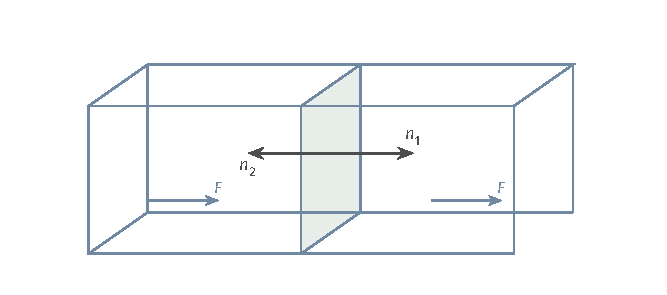
\includegraphics[width=112mm]{figures/01-mathematical-preliminaries-upper/01-mathematical-language-combinatorics-analysis-optimization/tikz/chapter3-concept-processes/gauss-shared-face.pdf}
 \caption{两个相邻单位立方体共用绿色面，图用斜投影表示三维几何。取常场$F=(1,0,0)^\top$，共同面上两侧外法向为$n_1=(1,0,0)^\top$与$n_2=-n_1$，对应通量为$1,-1$，相加抵消。整体外向净通量也为零，与散度为零一致；一般区域的散度定理仍需要前述条件与证明。}
 \label{fig:analysis-process-gauss-shared-face}
\end{figure}

例如半径$R>0$的球面取外法向，令$\bm F(\bm x)=\bm x/R$。球面上$\bm F=\bm n$，故通量也等于球面积。
由于$\operatorname{div}\bm F=3/R$，散度定理给出
\[
 \int_{\partial B_R}\bm F^\top\bm n\,\mathrm dS
 =\frac3R\operatorname{vol}(B_R)
 =\frac3R\frac{4\pi R^3}3=4\pi R^2.
\]
这里的球体积可由圆盘截面积分得到，结果与前面直接参数化球面求面积一致。

\subsubsection{多元分部积分}

一元分部积分把一个因子的导数转给另一个因子，并留下端点项。
在多元情形中，对乘积向量场使用散度公式，就得到相应的边界通量项。
\begin{theorem}[多元分部积分]
\label{thm:multivariable-integration-by-parts}
设$\Omega\subseteq\mathbb R^3$满足上述Gauss公式的区域条件。
若标量函数$u$在$\overline\Omega$的开邻域内连续可微，$v$在同一邻域内二阶连续可微，则
\[
 \int_\Omega u\Delta v\,\mathrm d\bm x
 =\int_{\partial\Omega}u\nabla v^\top\bm n\,\mathrm dS
  -\int_\Omega\nabla u^\top\nabla v\,\mathrm d\bm x.
\]
\end{theorem}
\begin{proof}
向量场$\bm F=u\nabla v$连续可微，逐坐标的乘积法则给出
\[
 \operatorname{div}(u\nabla v)
 =\nabla u^\top\nabla v+u\Delta v.
\]
将它代入Gauss公式，再把第一项的区域积分移到等式另一侧，即得结论。
\end{proof}
对满足Green公式条件的平面区域，同样的证明使用平面通量公式即可成立，边界面积元素相应换成弧长元素。
这一公式把$v$的二阶导数转移为$u$与$v$的一阶导数，同时保留法向边界项；该项是否为零，必须由具体边界条件决定。

\subsection{曲面积分与边界路径积分}

Gauss公式要求闭曲面围成空间区域。另一类问题只给一张有边界的定向曲面，要求比较曲面上的旋转累计与边界环流。
这时应使用旋度在曲面法向上的分量，不需要先把曲面补成闭曲面。

\subsubsection{Stokes公式}

在$z=0$平面上取向上法向时，旋度的法向分量就是Green公式中的$Q_x-P_y$。
Stokes公式将这一关系推广到空间中的定向曲面，同时要求法向与边界方向相容。
\begin{theorem}[Stokes定理]
\label{thm:multivariable-stokes}
设$S\subseteq\mathbb R^3$为紧致、可定向的分片$C^2$曲面，边界由有限条分段$C^1$简单闭曲线组成。
各光滑曲面片选取连续且片间定向相容的单位法向$\bm n$，边界采用其诱导方向。
若向量场$\bm F$在$S$的开邻域内连续可微，则\term{Stokes公式}（Stokes' theorem）给出
\begin{equation}
 \oint_{\partial S}\bm F^\top\,\mathrm d\bm r
 =\int_S(\nabla\times\bm F)^\top\bm n\,\mathrm dS.
 \label{eq:multivariable-stokes}
\end{equation}
\end{theorem}
这里的“可定向”要求各曲面片能相容地选择法向，使公共边上的诱导方向相反；有折角的接缝处不要求存在唯一法向。
两侧都为标量：左侧是原向量场的边界环流，右侧是其旋度穿过曲面的通量。

在一张参数曲面片上，可以把公式归结为参数平面上的Green公式。
设$\bm r(u,v)$在规则参数域$D$的邻域内二阶连续可微、在内部正则且一一对应，并采用$\bm r_u\times\bm r_v$确定的定向。
还要求参数边界按诱导方向对应曲面片的边界，从而可以沿$\partial D$计算边界路径积分。
记
\[
 \begin{aligned}
 A(u,v)&=\bm F(\bm r(u,v))^\top\bm r_u(u,v),\\
 B(u,v)&=\bm F(\bm r(u,v))^\top\bm r_v(u,v).
 \end{aligned}
\]
边界路径的链式法则将左侧变成$\oint_{\partial D}A\,\mathrm du+B\,\mathrm dv$。
对$A,B$逐项求偏导，含$\bm r_{uv}$与$\bm r_{vu}$的项因混合偏导相等而相消，剩下
\[
 \partial_uB-\partial_vA
 =\bigl(\operatorname{curl}\bm F\bigr)(\bm r(u,v))^\top
   (\bm r_u\times\bm r_v).
\]
参数平面上的Green公式因此给出该曲面片上的Stokes公式。
对有限张相容定向的曲面片，公共边的路径积分相消，只剩整张曲面的边界。
一般分片曲面的完整论证还需核对曲面覆盖及接缝条件，以上推导说明参数片上的机制；一般定理可参考所引教材\scite{math-strang1991calculus}。

\subsubsection{跨接曲面的选择}

Stokes公式的边界积分只由有向边界和边界上的向量场决定。因此，若两张满足定理条件的定向曲面具有同一有向边界，
且$\bm F$在两张曲面附近都连续可微，则两张曲面上的旋度通量相等。
计算时可以选较简单的跨接曲面，但必须核对向量场定义域，不能让替换曲面穿过场的奇点。

例如$\bm F=(-y/2,x/2,0)^\top$有$\nabla\times\bm F=(0,0,1)^\top$。
单位圆采用从上方看逆时针的方向，取向上单位圆盘$S$，便有
\[
 \oint_{\partial S}\bm F^\top\,\mathrm d\bm r
 =\iint_S1\,\mathrm dS=\pi.
\]
上半球面取外法向时，边界诱导方向相同，旋度通量仍为$\pi$。
若改用向下定向的圆盘，边界方向也必须反转，两个积分同时变号。


图~\ref{fig:analysis-process-stokes-spanning-surfaces}比较同一有向圆周的两张跨接曲面。替换曲面时，边界方向与场的定义域都要同时保留。
\begin{figure*}[!htbp]
 \centering
 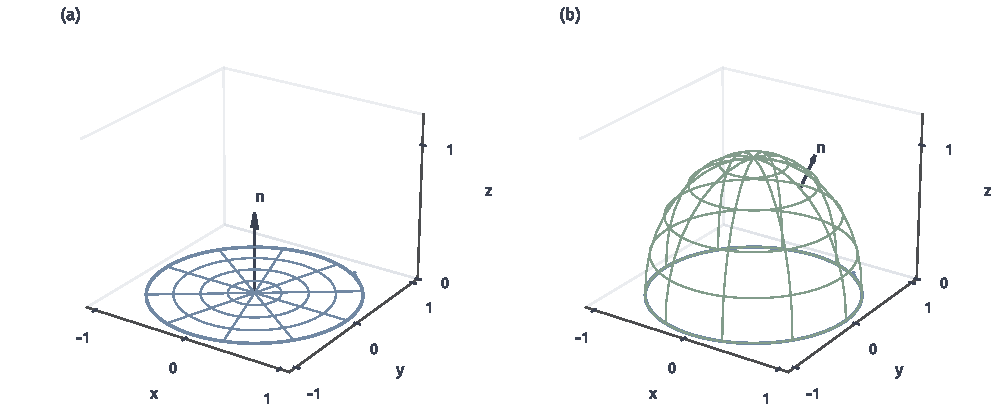
\includegraphics[width=169.0mm]{figures/01-mathematical-preliminaries-upper/01-mathematical-language-combinatorics-analysis-optimization/matplotlib/chapter3-concept-processes/stokes-spanning-surfaces.pdf}
 \caption{(a) 向上单位圆盘；(b) 外向上半单位球面。蓝色边界均从上方看逆时针，黑箭头标记各自法向。对$F=(-y/2,x/2,0)^\top$，旋度恒为$(0,0,1)^\top$，两面上的旋度通量都为$\pi$。右面面积为$2\pi$而非$\pi$；相等的是法向分量的累计，不能把通量当成面积。}
 \label{fig:analysis-process-stokes-spanning-surfaces}
\end{figure*}

\subsection{积分公式的比较}

前面的公式回答的都是导数在内部的积分与边界积分之间的关系，但内部对象、边界对象和方向条件各有不同。
一元基本定理以区间两端为边界；梯度场的路径积分基本定理以路径两端为边界。这里进一步得到下面三种关系。
\begin{center}
\begin{tabular}{lll}
\toprule
公式 & 内部积分 & 边界积分\\
\midrule
Green环流形式 & 平面区域的$Q_x-P_y$ & 正向路径的切向积分\\
Gauss & 空间区域的散度 & 闭曲面的外向通量\\
Stokes & 定向曲面的旋度通量 & 诱导方向的路径环流\\
\bottomrule
\end{tabular}
\end{center}
对向上定向的平面曲面，Stokes公式还原Green公式的环流形式；
Green公式的通量形式则是二维的散度公式。
普通标量函数的区域积分不自动具有边界表达：要使用这些公式，须先找到满足条件的向量场，使其散度或旋度的相应分量等于被积函数。

各公式均使用勒贝格积分。连续可微性、分片规则边界与定向是这里的经典公式所需的条件，并不是另换一种积分定义。
尤其要核对向量场是否在整个积分对象附近都有定义：前面穿孔平面上的场在原点无定义，就不能把包含原点的圆盘直接代入Green公式。
仅知道两个函数在体积测度下几乎处处相等，也不足以确定其边界积分，因为边界本身可以是体积零测集。
如果要降低导数或边界的规则性，还须另外建立弱导数、边界迹及相应的积分公式；不能沿用当前公式而省去这些条件。

\FloatBarrier
